\chapter{Methods}
\label{methods}
In the following chapter, we are going to elaborate on how we performed the experiments, which hyperparameters where used and how we evaluated the results of the trained models.

\section{Architecture of the Sequence-To-Sequence Model}
In the following paragraphs, we are going to describe the architecture of the model used to conduct our experiments.

\paragraph{Sequence-To-Sequence} In general, we are using the architecture of seq2seq models describe in chapter \ref{fundamentals:seq2seq} with LSTM cells. We restrict ourselves to only use one LSTM cell for the encoder, and another cell for the decoder. This has to do with the fact, that we wanted our cells to be as large as possible to come as close to the size of the cells used in \cite{Vinyals:2015}. However, this is not simply possible due to the fact, that in the referenced paper they used two really large cells with each having a hidden state size of $4096$ hidden units and a vocabulary consisting of $100'000$ words. In the paper, they trained their models on a large number of CPUs due to this fact, because such a huge network fits does not fit in the memory of any GPU currently available. As we are seeking to train our models on a single GPU (see chapter \ref{sofware_system:development_history}), we had to shrink the size of our model to the biggest size possible so that it still fits within the 12GB of memory the GPUs we are using have (see chapter \ref{software_system:hardware}). The exact size of the model used in this thesis is described in the subsequent paragraph ``Hyperparameters'' below.

\paragraph{Down-Projection of Hidden State} Because of the problematic with such large RNN cells as described in the preceding paragraph, we implemented a so-called \emph{down-projection} at the end of the decoder cell. This is done similar to the down-projection used in \cite{Vinyals:2015}, with the main difference lying in the motivation why we implemented it. In the paper, they state, that they used it to speed up the training due to the large weights-matrix in the softmax layer at the end. In our case, the down-projection was not just for speeding up the training, but mainly to allow us to use larger cells than we would be able to without the projection. The implementation of this feature allowed us to grow our model in size by a factor of two, from a hidden state size of $1024$ to $2048$, without the need to sacrifice the size of the vocabulary used (see chapter \ref{methods:hyperparameters} for more information on the used hyperparameters).

\paragraph{Sampled Softmax} To speed up the training of the large softmax layer at the end (consisting of $50'000$ entries), we use a \emph{sampled softmax} as described in \cite{Sebastien:2014} which is only applied while training the models. Basically, the idea behind it is, that instead of using the full softmax at each time step in the decoder, we only use a subset of the words which is randomly sampled (besides the words which is the target word) from the vocabulary to approximate the softmax layer. This speeds up training dramatically due to the fact, that not the whole softmax layer has to be used and hence not all derivates have to be computed. On inference time, when we generate predictions, we have to use the full softmax layer again to generate the predictions.

\paragraph{Static Unrolling of RNN} Due to the fact, that we are working with a deprecated \texttt{TensorFlow} API (see chapter \ref{sofware_system:development_history}), we have to use static unrolling for our model. Static unrolling works, by defining a fixed size of time steps for the encoder and decoder, and then unrolling the encoder and decoder cell for this number of time steps \emph{before} we are actually computing anything using it. This actually ``removes'' the recurrence from our model and transforms it into kind-of ``feed forward'' model with the major difference being, that the weights are shared between the layers of the unrolled model (as each layer basically represents the same cell). With the latest \texttt{TensorFlow} API\footnote{https://www.tensorflow.org/api\_docs/python/tf/nn/dynamic\_rnn}, it is possible to create the graph for the encoder dynamically at runtime based on the length of the input. The decoder, in the dynamic case, then runs for as many time steps as necessary to either reach an \texttt{EOS} token or the maximum number of time steps allowed to decode.

\begin{figure}
	\label{methods:static_unrolling:unrolled_rnn}
	\centering
	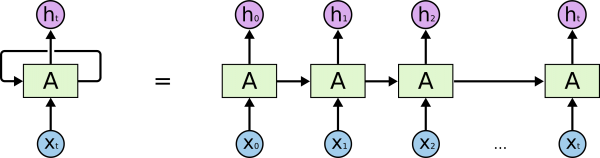
\includegraphics[width=10cm]{img/rnn_unrolled}
	\caption{Image for illustrating the process of unrolling an RNN over a fixed size of time steps.\protect\footnotemark}
\end{figure}
\footnotetext{http://colah.github.io/posts/2015-08-Understanding-LSTMs/}

This implementation forced us to define a maximum number of time steps used for the encoder and decoder beforehand, which we have set to $30$ for both the encoder and decoder. This length is also mainly restricted due to the fact, that the longer timespan we pick, the larger the memory consumption on the GPU becomes. We tried several different sizes ranging from $10$ to $100$ time steps and evaluated that $30$ would be the largest possible size without the need to shrink any other parts of the model.

\paragraph{Reversing the Input Sequence} As \cite{Sutskever:2014} have noticed in their paper, it was beneficial to reverse the input sequence before feeding it to the model. They assume, that this helps because the minimal time lag \cite{Hochreiter:1997} is greatly reduced due to the fact that the first few words in the source language are much closer to the first few words in the target language. This explanation makes sense in the context of machine translations, but not necessarily in the context of a conversational dialog-system. Nevertheless, we want to try to use it and see if it makes any difference our models. We decided that the Reddit model should be the one that is trained with reversed input sequences.

\section{OpenSubtitles and Reddit Models}
\label{methods:both_models}
As already described in chapter \ref{chapter:data}, we are going to train two distinct models that each use a separate training, validation and test corpus. The first is trained on the OpenSubtitles corpus and the second on the Reddit corpus. Both of them are going to be trained in the same way for the same time, except for the difference regarding how the input sequences are fed to the model.

\section{Hyperparameters}
\label{methods:hyperparameters}

\paragraph{Model} The hyperparameters used for training the models can be seen in table \ref{methods:hyperparameters:table}. Both of our models use the same set of hyperparameters, the only difference being that the Reddit model is fed with reversed input sequences whereas the OpenSubtitles model is not.

\begin{table}[H]
	\centering
	\ra{1.3}
	\begin{adjustbox}{max width=\textwidth}
		\begin{tabular}{ll}
			\toprule
			Name & Value\\ \midrule
			Number of encoder cells & $1$\\
			Number of decoder cells & $1$\\
			Max. number of time steps in encoder & $30$\\
			Max. number of time steps in decoder & $30$\\
			Hidden state size & $2048$\\
			Projected hidden state size & $1024$\\
			Number of sampled words for softmax & $512$\\
			Size of the softmax layer & $50'000$\\
			Batch size & $64$\\
			\bottomrule
		\end{tabular}
	\end{adjustbox}
	\caption{Hyperparameters used for our seq2seq models.}
	\label{methods:hyperparameters:table}
\end{table}

\paragraph{Optimizer} As the optimizer, we use \emph{AdaGrad} \cite{Duchi:2011} as in \cite{Vinyals:2015} with the learning rate set to $0.01$. We also use gradient clipping and set the maximum allowed gradient value to be $10$, as described in \cite{Pascanu:2013}.

\paragraph{Training} We train our models on the hardware described in chapter \ref{software_system:hardware} with the software packages from chapter \ref{software_system:softwar_packages}. As this models take a really long time to converge (in \cite{Vinyals:2015} the authors trained their model for several weeks), we also have to train ours for a long time. To show the development of the model throughout this time, we took several snapshots, approximately every third day or about after every 500'000 batches. The taken snapshots are going to be used in the analysis we are going to do in the next chapter. They enable us to not only do an analysis of the final results, but rather show the evolution of the models throughout the training process. The two models were trained over a time period of 20 days, each trained on 3 million batches, each containing 64 samples.

As the two training datasets are not equal in size, using the same time period for the training of both models induces that they see different shares of their respective training datasets. In the case of the OpenSubtitles model, the case is that it can only process 192 million samples, which equals to about 59\% percent of the whole OpenSubtitles training corpus. In the case of the Reddit model, the two week training allows doing two and a half epochs over the entire dataset. This allows us to analyse the difference between using the approaches of using a single big corpus, which we are not able to completely process, against a smaller corpus that we can iterate more than twice in the same time.

\section{Evaluation}
We use two different kinds of evaluation: Metric-based and human-based. The first one is a quantitative analysis of the results and consists of analyzing the training process and the final results under the metrics defined in Chapter~\ref{fundamentals:metrics}. We are also going to do an n-gram analysis, as already mentioned in Chapter~\ref{chapter:data:ngram}, where we analyze the language model of the resulting models with regard to the language used in the corpora. This also includes an analysis of the syntax and semantics of the outputs generated by the trained models. The human evaluation is done by judging how ``meaningful'' the texts generated by the resulting model are and we compare them with results found in other papers (e.g. \cite{Vinyals:2015}) and chatbots (such as CleverBot\footnote{http://www.cleverbot.com/}).

We also considered using the BLEU and ROGUE metrics for evaluating our models. After some research, we have found that this metrics are primarily used in the context of machine translations and work by comparing the resulting texts to several reference translations. In our opinion, this does not make a lot of sense in the context of conversational models since the answers to a specific input can have a wide variety of possible forms that are all meaningful and fitting but do not necessarily to be alike the reference output. This thought is supported by results that Nguyen et al. \cite{Nguyen:2016} have found in their paper, where they state that they used the BLEU and ROGUE metrics for evaluating their chatbot and determined that these metrics are not fit to do such an evaluation because of the aforementioned reasons. Instead of the mentioned similarity metric, we are going to use Sent2Vec~\cite{Pgj:2017}, which allows us to do similarity measures between the expected and generated outputs of the model using a highly dimensional vector space where the sequences can be embedded. This can be done by using the pretrained models found in the GitHub repository\footnote{https://github.com/epfml/sent2vec}, as it is possible to embed new sequences without the requirement of retraining the models.
